%!TEX encoding = UTF-8 Unicode
%!TEX root = ../lect-w10.tex

%%%


%\begin{Slide}{TODO: Begrepp att förklara}
%  Tänk igenom ordningen:
%  \begin{itemize}
%    \item OO, arv, supertyp, subtyp, bastyp, polymorfism, ...
%  \end{itemize}
%\end{Slide}


\Subsection{Överskuggingsregler, \texttt{override}}

\begin{Slide}{Medlemmar, arv och överskuggning}\SlideFontTiny
\begin{multicols}{2}
\noindent Olika sorters överskuggningsbara medlemmar i \Emph{Scala}:
\begin{itemize}
\item \code{def}
\item \code{val}
\item \code{lazy val}
\item \code{var}
\end{itemize}


\columnbreak

\pause

\noindent Olika sorters överskuggningsbara instansmedlemmar i \Emph{Java}:
\begin{itemize}
\item variabel
\item metod
\end{itemize}

{\SlideFontTiny\noindent Medlemmar som är \jcode{static} kan ej överskuggas (men döljas) vid arv.}

\vspace{0.5em}
\end{multicols}

\pause
\begin{itemize}\SlideFontTiny
\item När man överskuggar \Eng{override} en medlemmen med en annan medlem med samma namn i en subtyp, får denna medlem en (ny) implementation.

\item När man konstruerar ett objektorienterat språk gäller det att man definierar sunda överskuggningsregler vid arv. Detta är förvånansvärt knepigt.

\item Singelobjekt kan ej ärvas (och medlemmar i singelobjekt kan därmed ej överskuggas).
\end{itemize}
\end{Slide}


\begin{Slide}{Fördjupning: Regler för överskuggning i Scala} \SlideFontTiny
\label{slideW07:overriderules}
En medlem M1 i en supertyp får överskuggas av en medlem M2 i en subtyp, enligt dessa regler:
\begin{enumerate}
\item M1 och M2 ska ha samma namn och typerna ska matcha.
\item \code{def} får bytas ut mot: \code{def}, \code{val}, \code{var}, \code{lazy val}
\item \code{val} får bytas ut mot: \code{val}, och om M1 är abstrakt mot en \code{lazy val}.
\item \code{var} får bara bytas ut mot en \code{var}.
\item \code{lazy val} får bara bytas ut mot en \code{lazy val}.
\item Om en medlem i en supertyp är abstrakt \emph{behöver} man inte använda nyckelordet \code{override} i subtypen. (Men det är bra att göra det ändå så att kompilatorn hjälper dig att kolla att du verkligen överskuggar något.)
\item Om en medlem i en supertyp är konkret \emph{måste} man använda nyckelordet \code{override} i subtypen, annars ges kompileringsfel.
\item M1 får inte vara \code{final}.
\item M1 får inte vara \code{private} eller \code{private[this]}, men kan vara \code{private[X]} om M2 också är \code{private[X]}, eller \code{private[Y]} om X innehåller Y.
\item Om M1 är \code{protected} måste även M2 vara det.

\end{enumerate}
\end{Slide}


\Subsection{\texttt{super}}

\begin{Slide}{Att skilja på mitt och ditt med \texttt{super}}
\begin{REPL}
scala> class X { def gurka = "super pepino" }

scala> class Y extends X {
         override val gurka = ":("
         val sg = super.gurka
       }

scala> val y = new Y
y: Y = Y@26ba2a48

scala> y.gurka
res0: String = :(
\end{REPL}

\pause
Super Pepinos to the rescue:
\begin{REPLnonum}
scala> y.sg
res1: String = super pepino

\end{REPLnonum}


\pause
\begin{tikzpicture}[overlay]
     \node at (7.5,1.7) {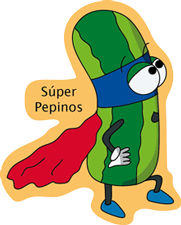
\includegraphics[scale=0.5]{../img/ttsuper}};
\end{tikzpicture}
\href{https://youtu.be/NPhjiXskz34}{\small https://youtu.be/NPhjiXskz34}
%\href{http://www.pepinadas.com/}{\small www.pepinadas.com/}
\end{Slide}




\Subsection{Trait eller abstrakt klass?}

\begin{Slide}{Trait eller abstrakt klass?}
\SlideFontSmall
\label{slideW07:traitorclass}
\begin{multicols}{2}
\noindent Använd en \Emph{trait} som supertyp om...
\begin{itemize}
\item ...du är osäker på vilket som är bäst. (Du kan alltid ändra till en abstrakt klass senare.)
\item ...du vill kunna mixa in din trait tillsammans med andra traits.
\item ...du vill göra din typ transparent vid typhärledning.
%\item ...du vill skapa ett flexibelt gränssnitt som del i ett api.

\end{itemize}

\columnbreak

\noindent Använd en \Alert{abstrakt klass} som supertyp om...
\begin{itemize}
%\item ...du vill ge supertypen en parameter vid konstruktion. \footnote{I kommande Scala 3 kan traits ha parametrar.}
\item ...du vill ärva supertypen från klasser skrivna i Java.
\item ...du vill minimera vad som behöver omkompileras vid ändringar.
\end{itemize}


\end{multicols}
\end{Slide}



% \begin{Slide}{Uppräknade värden med case-objekt}\SlideFontSmall
% Vi kan använda case-objekt och arv för att representera olika färger.
% \begin{Code}[language=,keywords={sealed,trait,object,case,class,extends}]
% sealed trait Färg
% case object Spader  extends Färg
% case object Hjärter extends Färg
% case object Ruter   extends Färg
% case object Klöver  extends Färg

% case class Kort(färg: Färg, valör: Int)
% \end{Code}

% Vi kan nu använda våra uppräknade färgvärden så här:
% \begin{REPL}
% scala> Kort(Ruter, 7)

% scala> Kort(Spader, 1)
% \end{REPL}
% \begin{itemize}
% \item Kompilatorn \Emph{garanterar} att vi bara använder exakt dessa färger.

% \item Nyckelordet \code{sealed} förhindrar fler subtyper förutom de som finns här.

% \item \code{case} före \code{object} ger en najs \code{toString} och möjliggör matchning \\
% (mer om matchning i w10).

% \end{itemize}

% \end{Slide}

% \begin{Slide}{Uppräknade värden i samling}\SlideFontSmall
% Vi kan placera case-objekten i en samling som kan användas i loopar. \\ Ett lämpligt ställe för en sådan samling är i kompanjonsobjektet till \code{Färg}.
% \begin{Code}
% sealed trait Färg
% object Färg {
%      val values = Vector(Spader, Hjärter, Ruter, Klöver)
% }
% case object Spader extends Färg
% case object Hjärter extends Färg
% case object Ruter extends Färg
% case object Klöver extends Färg
% \end{Code}

% \begin{REPL}
% scala> val allaEss = for (f <- Färg.values) yield Kort(f, 1)
% \end{REPL}
% \end{Slide}

% \begin{Slide}{Uppräknade värden med heltal}\SlideFontSmall
% Vi kan använda heltalskonstanter för att representera olika färger.
% \begin{Code}
% object Färg {
%   val Spader = 1
%   val Hjärter = 2
%   val Ruter = 3
%   val Klöver = 4
% }
% \end{Code}
% \begin{Code}[language=,keywords={case,class}]
% case class Kort(färg: Int, valör: Int)
% \end{Code}

% Vi kan nu använda våra uppräknade färgvärden så här:
% \begin{REPLnonum}
% scala> import Färg._
% scala> Kort(Ruter, 7)
% \end{REPLnonum}
% \pause Men kompilatorn \Alert{kan inte hindra} denna bugg:
% \begin{REPLnonum}
% scala> Kort(42, 7)
% \end{REPLnonum}

% \end{Slide}



\begin{Slide}{Förseglade typer med \texttt{sealed}}\SlideFontSmall
Med en \code{sealed} kan du skapa en \Emph{förseglad} datatyp, exempel uppräkning:
\begin{Code}
sealed trait Färg(val toInt: Int)
object Färg:
  val values = Vector(Spader, Hjärter, Ruter, Klöver)

  case object Spader  extends Färg(0)
  case object Hjärter extends Färg(1)
  case object Ruter   extends Färg(2)
  case object Klöver  extends Färg(3)
\end{Code}
Nyckelordet \code{sealed} förhindrar vidare subtypning av \code{Färg} och ger varning om matchning inte är fullständig, vilket är till stor hjälp för att förhindra buggar.

\begin{REPL}
scala> Färg.values(0) match { case Färg.Spader => "hej" }
-- Warning:
1 |Färg.values(0) match { case Färg.Spader => "hej" }
     |^^^^^^^^^^^^^^
     |match may not be exhaustive.
     |
     |It would fail on pattern case: Hjärter, Ruter, Klöver
val res0: String = hej
\end{REPL}
\end{Slide}




\begin{Slide}{Terminologi och nyckelord vid arv}\SlideFontTiny

\begin{tabular}{r  l}
\Emph{subtyp}           & en typ som ärver en supertyp\\
\Emph{supertyp}         & en typ som ärvs av en subtyp\\
\Emph{bastyp}           & en typ som är rot i ett arvsträd\\
\Emph{abstrakt medlem}  & en medlem som saknar implementation\\
\Emph{konkret medlem}   & en medlem som ej saknar implementation\\
\Emph{abstrakt typ}     & en typ som kan ha abstrakta medlemmar; kan ej instansieras\\
\Emph{konkret typ}      & en typ som ej har abstrakta medlemmar; kan instansieras\\
\code|class|            & en klass är en konkret typ: \Alert{kan ej ha abstrakta medlemmar}\\
\code|abstract class|   & en klass är en abstrakt typ som \Emph{kan ha parametrar}\\
\code|trait|            & är en abstrakt typ, \Alert{kan ej ha parametrar} men \Emph{kan mixas in}\\
\code|extends|          & står före en supertyp, medför arv av supertypens medlemmar\\
\code|override|         & en medlem överskuggar (byter ut) en medlem i en superttyp\\
\code|protected|        & gör en medlem synlig i subtyper till denna typ (jmf \code|private|)\\
\code|final gurka|      & gör medlemen gurka final: förhindrar överskuggning\\
\code|final class|      & gör klassen final: förhindrar vidare subtypning\\
\code|sealed trait|     & förseglad trait: bara de direkta subtyperna i denna kodfil\\
\code|super.gurka|      & refererar till supertypens medlem \code|gurka| (jmf \code|this|)\\
\end{tabular}

\ifkompendium\else
\pause
\begin{tikzpicture}[overlay]
     \node at (10.7,0.6) {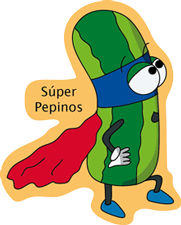
\includegraphics[scale=0.36]{../img/ttsuper}};
\end{tikzpicture}
\fi

\end{Slide}



\Subsection{Datatyper}

\begin{Slide}{Terminologi för datatyper}\SlideFontSmall
\begin{itemize}
\item Abstrakt datatyp \Eng{abstract data type}
\begin{itemize}\SlideFontTiny
\item Definieras av gränssnittet och beteendet -- implementationen är dold för användaren. 
\item Fördelar: inkapsling, lokala ändringar, flexibilitet.
\item Skapas i Scala t.ex. med klasser + privata medlemmar.
\end{itemize} 
\item Enumeration, ä.k. uppräkning \Eng{enumeration}
\begin{itemize}\SlideFontTiny
\item En speciellt enkel form av s.k. algebraisk datatyp som består av en uppräknad, ändlig sekvens av enkla värden som har en ordning.
\item Skapas i Scala med 1) heltal, 2) \code{sealed trait} ... \code{case class} ... 3) \code{enum}
\end{itemize} 
\item Algebraisk datatyp \Eng{algebraic data type}
\begin{itemize}\SlideFontTiny
\item En datatyp som är sammansatt av delar som kan kombineras. 
\item Två olika algebraiska datatyper som kan kombineras med varandra:
\begin{itemize}\SlideFontTiny
\item \Alert{Och}-typ (ä.k. produkttyp, record, struct), exempel: \\ \code|case class Person(namn: Int, ålder: Int)| \\består av attributen namn \Alert{OCH} ålder.
\item \Emph{Eller}-typ (ä.k. summatyp, unionstyp), exempel: \code|enum Färg { case Röd, Svart}| \\kan vara antingen röd \Emph{ELLER} svart.
\end{itemize}  
\end{itemize} 
\end{itemize}     
\end{Slide}


\begin{Slide}{Algebraiska datatyper}
     \TODO visa med både case classer och enum
\end{Slide}

\begin{Slide}{Unionstyper med eller-operator}
     \TODO
\end{Slide}